\documentclass{report}
\usepackage[utf8]{inputenc}
\usepackage{graphicx}
\usepackage[siunitx ,europeanresistors ,americaninductors]{circuitikz}
\usepackage{tikz}
\usepackage{pgfplots}
\graphicspath{{images/}}
\title{Vienkāršu elektrisku shēmu modelēšana}
\author{Mihails Linkevics}
\date{June 2018}

\begin{document}

\maketitle
\chapter{Teorētiskā daļa}
\section{Ķēdes aprēķins}
\begin{circuitikz}[scale=1, every node/.style={transform shape}]
\draw
(0,2) to[V=$V1$, ] (0,0)
(0,2) to[R=$R1$, -] (4,2)
(4,2) to[R=$R2$, -] (4,0)
(0,0) to[short, -] (4,0)
;
\end{circuitikz}
Apēķiniet spriegumus uz rezistoriem 1. attēlā dotajā shēmā. Sprieguma avota V1 sprieguma
vērtību U (Voltos) izvēlieties daļskaitli, kas būtu Jūsu apliecības pēdējie trīs cipari dalīti ar
10. Piemēram. ‘101REB123’ nozīmē V1 = 12.3 (Volti), R1 ir apliecības pēdējo 3 ciparu otrais
numurs+1, R2 ir apliecības numura pēdējais cipars +1. Piemēram, ja Jūsu apliecības numurs
ir ‘101REB123’ tad ‘R1=3’, ‘R2=4’. Nofotografējiet aprēķinu vai saglabājiet lapiņu. Aprēķina gaita
būs nepieciešama darbā ‘P02’. Turklāt, aprēķins būs jāpievieno atskaitei, ko veiksiet semestra
beigās. \cite{gramata1} \cite{gramata2}
\begin{flushleft}
V=184/10= 18.4 V
 
R1=8+1= 9 Ohm

R2=4+1= 5 Ohm
\end{flushleft}
\begin{flushleft}
I= V1/(R1+R2)=18.4/(9+5) = 1.31 A

UR1 =I*R1=9*1.31= 11,79 V

UR2 I*R2=5*1.31= 6.55 V
Izveidoju tabulu ar rezultātiem (\ref{Teoretiska tabula})
\end{flushleft}
\begin{table}
    \centering
    \begin{tabular}{c|c}
       \hline
R1 & 9 Ohm \\\hline
R2 & 5 Ohm \\\hline
V1 & 18.4 V \\\hline
UR1 & 11.79 V \\\hline
UR2 & 6.55 V \\\hline
    \end{tabular}
    \caption{Kedes elementu spriegumi un vertibas}
    \label{Teoretiska tabula}
\end{table}
\chapter{Praktiska dala}
\section{Darbs ar GEDA programmām}
\subsection{darbs ar gschem}
Ar GEDA komandu gschem izveidoju shemu\\(\ref{GEDA Shema})
(\ref{GEDA Shema})
\begin{figure}[!tb]
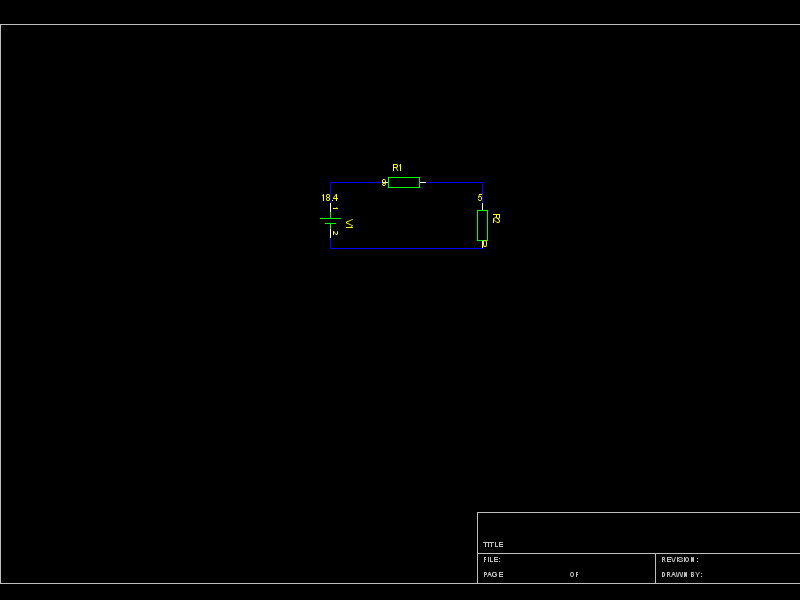
\includegraphics[width=\textwidth,height=\textheight,keepaspectratio]{IMAGES/01.png}
\caption{Elektriskā shēma no GEDA}
\label{GEDA Shema}
\end{figure}
\subsection{darbs ar gnetlist}
\begin{flushleft}
* Spice netlister for gnetlist

V1  2   0   18.4

R2  1   0   5

R1  2   1   9

.END
\end{flushleft}
\subsection{darbs ar ngspice}
Ar ngspice izveidoju divus grafikus. Att. (\ref{ngspice grafiks 1}) un (\ref{ngspice grafiks 2})
\begin{figure}[!tb]
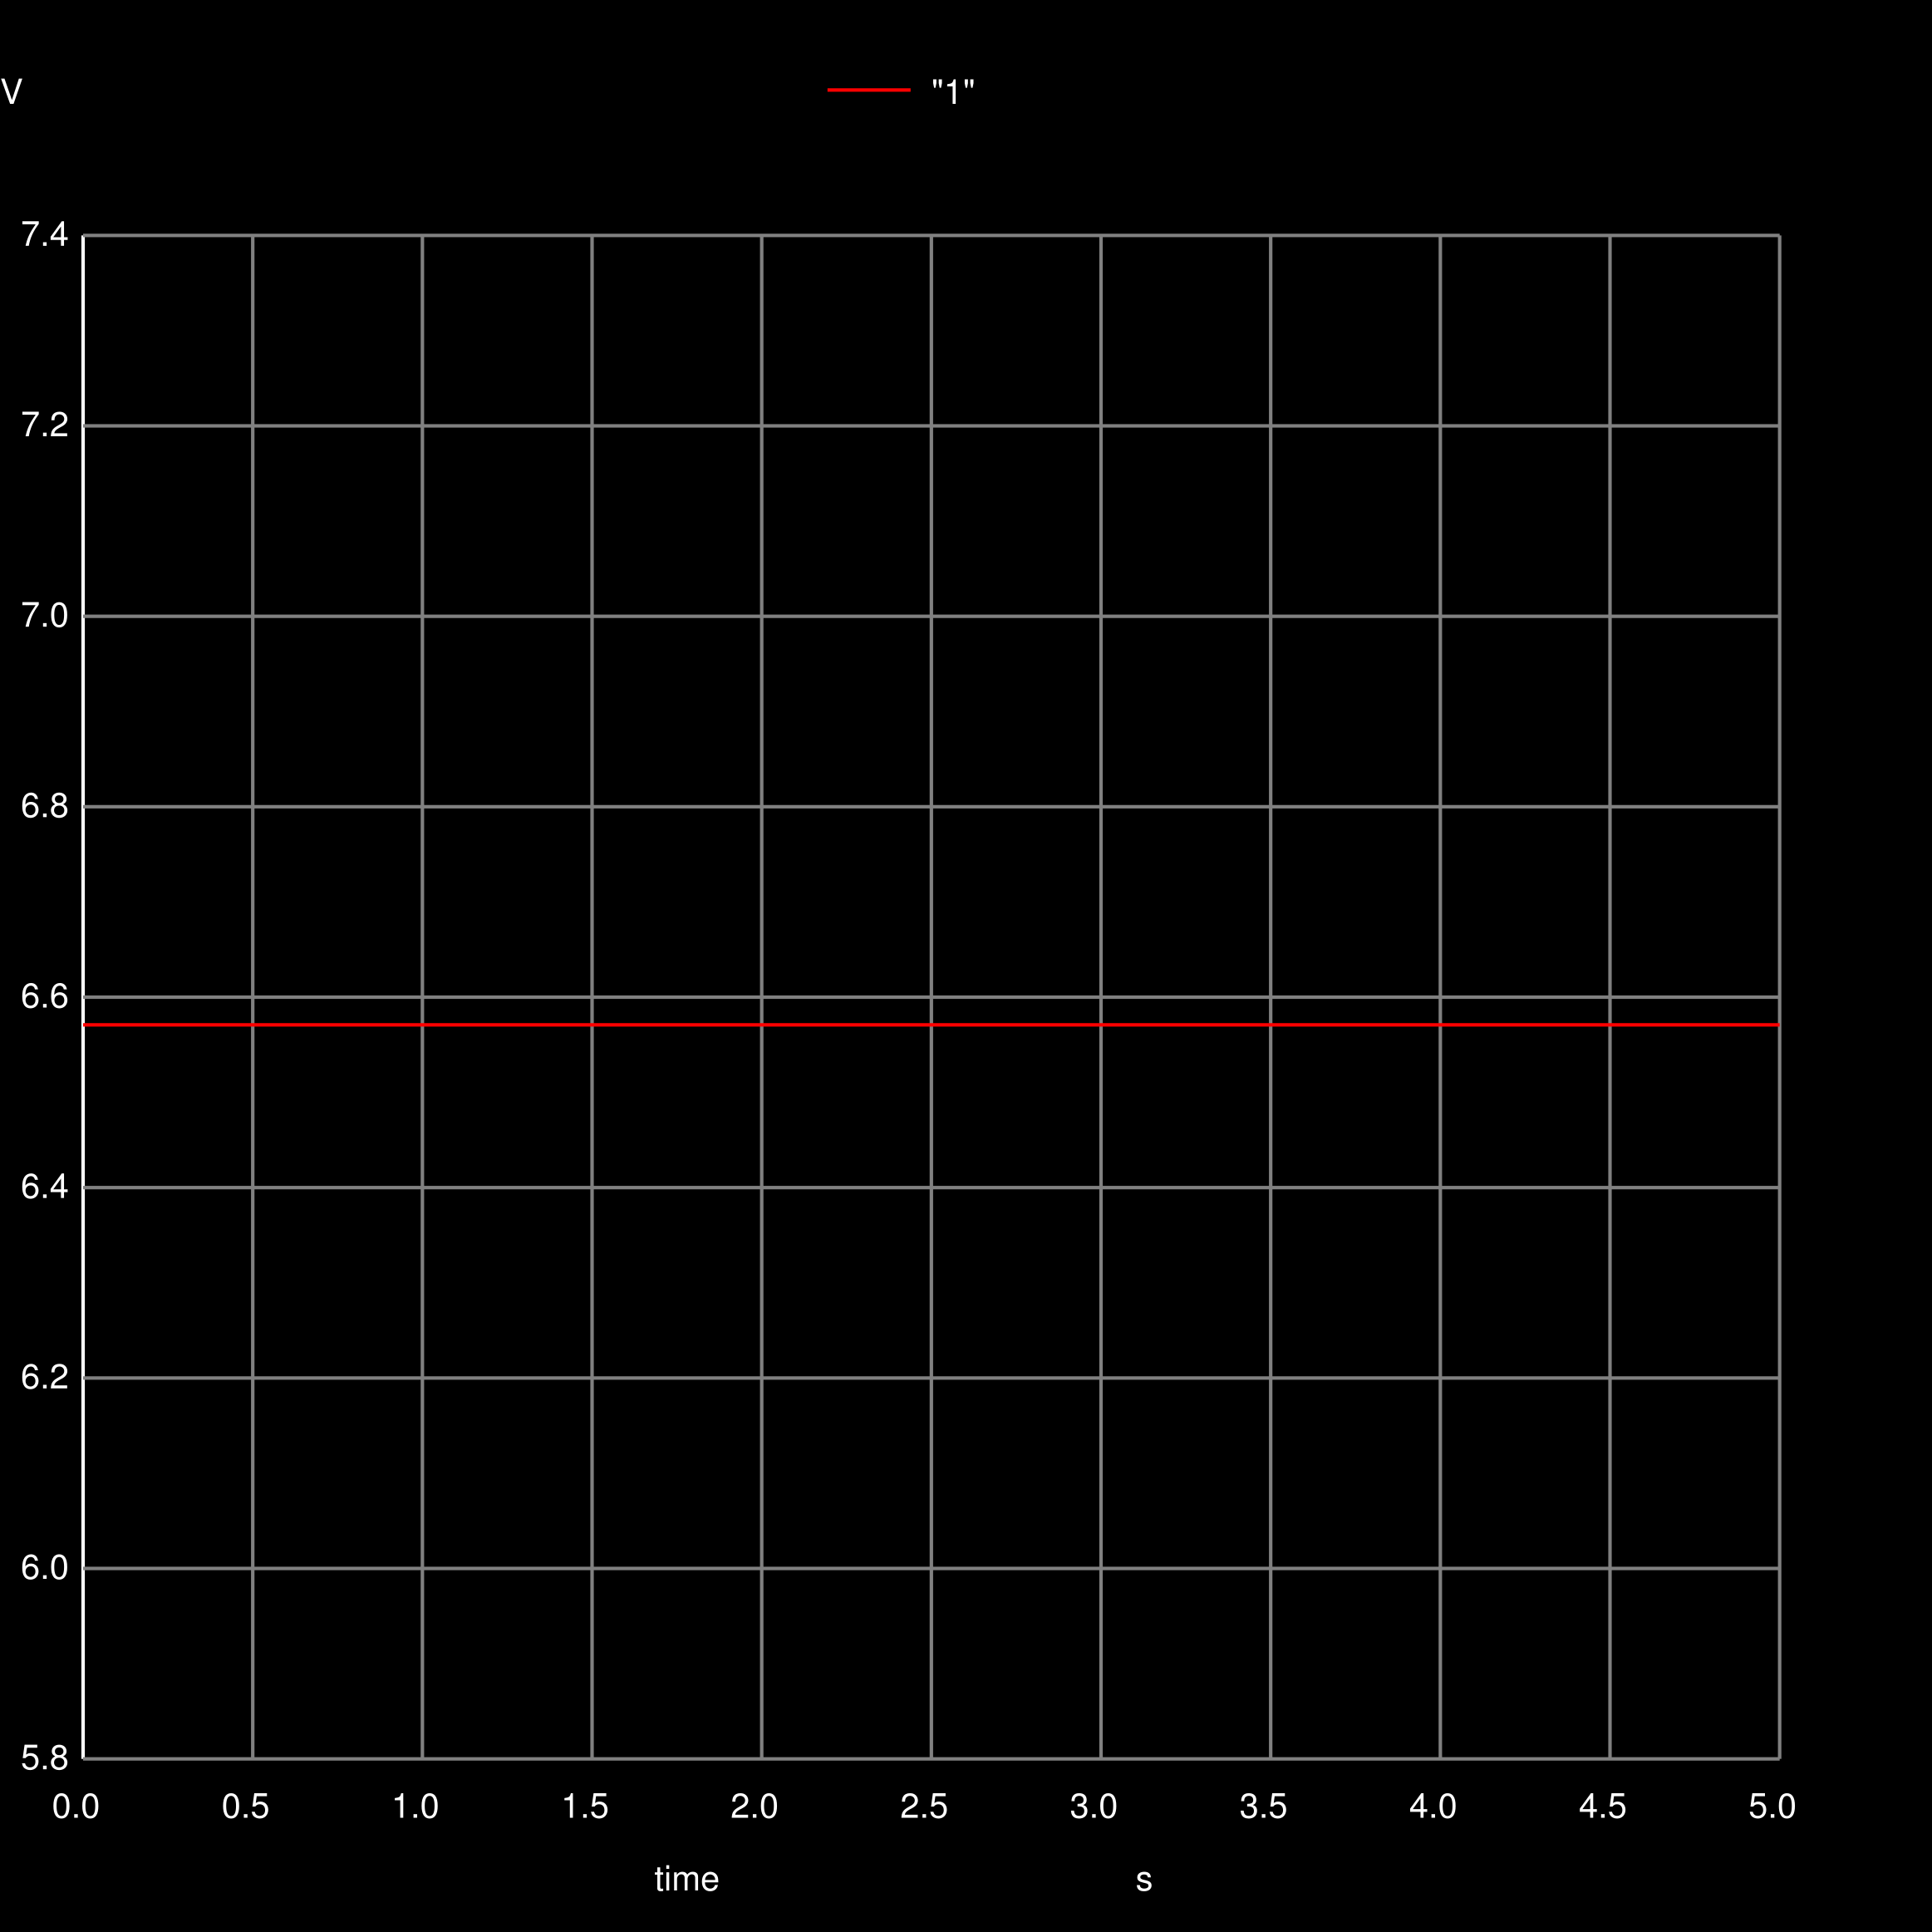
\includegraphics[width=\textwidth,height=\textheight,keepaspectratio]{IMAGES/011.png}
\caption{Grafiks no ngspice (1)}
\label{ngspice grafiks 1}
\end{figure}
\begin{figure}[!tb]
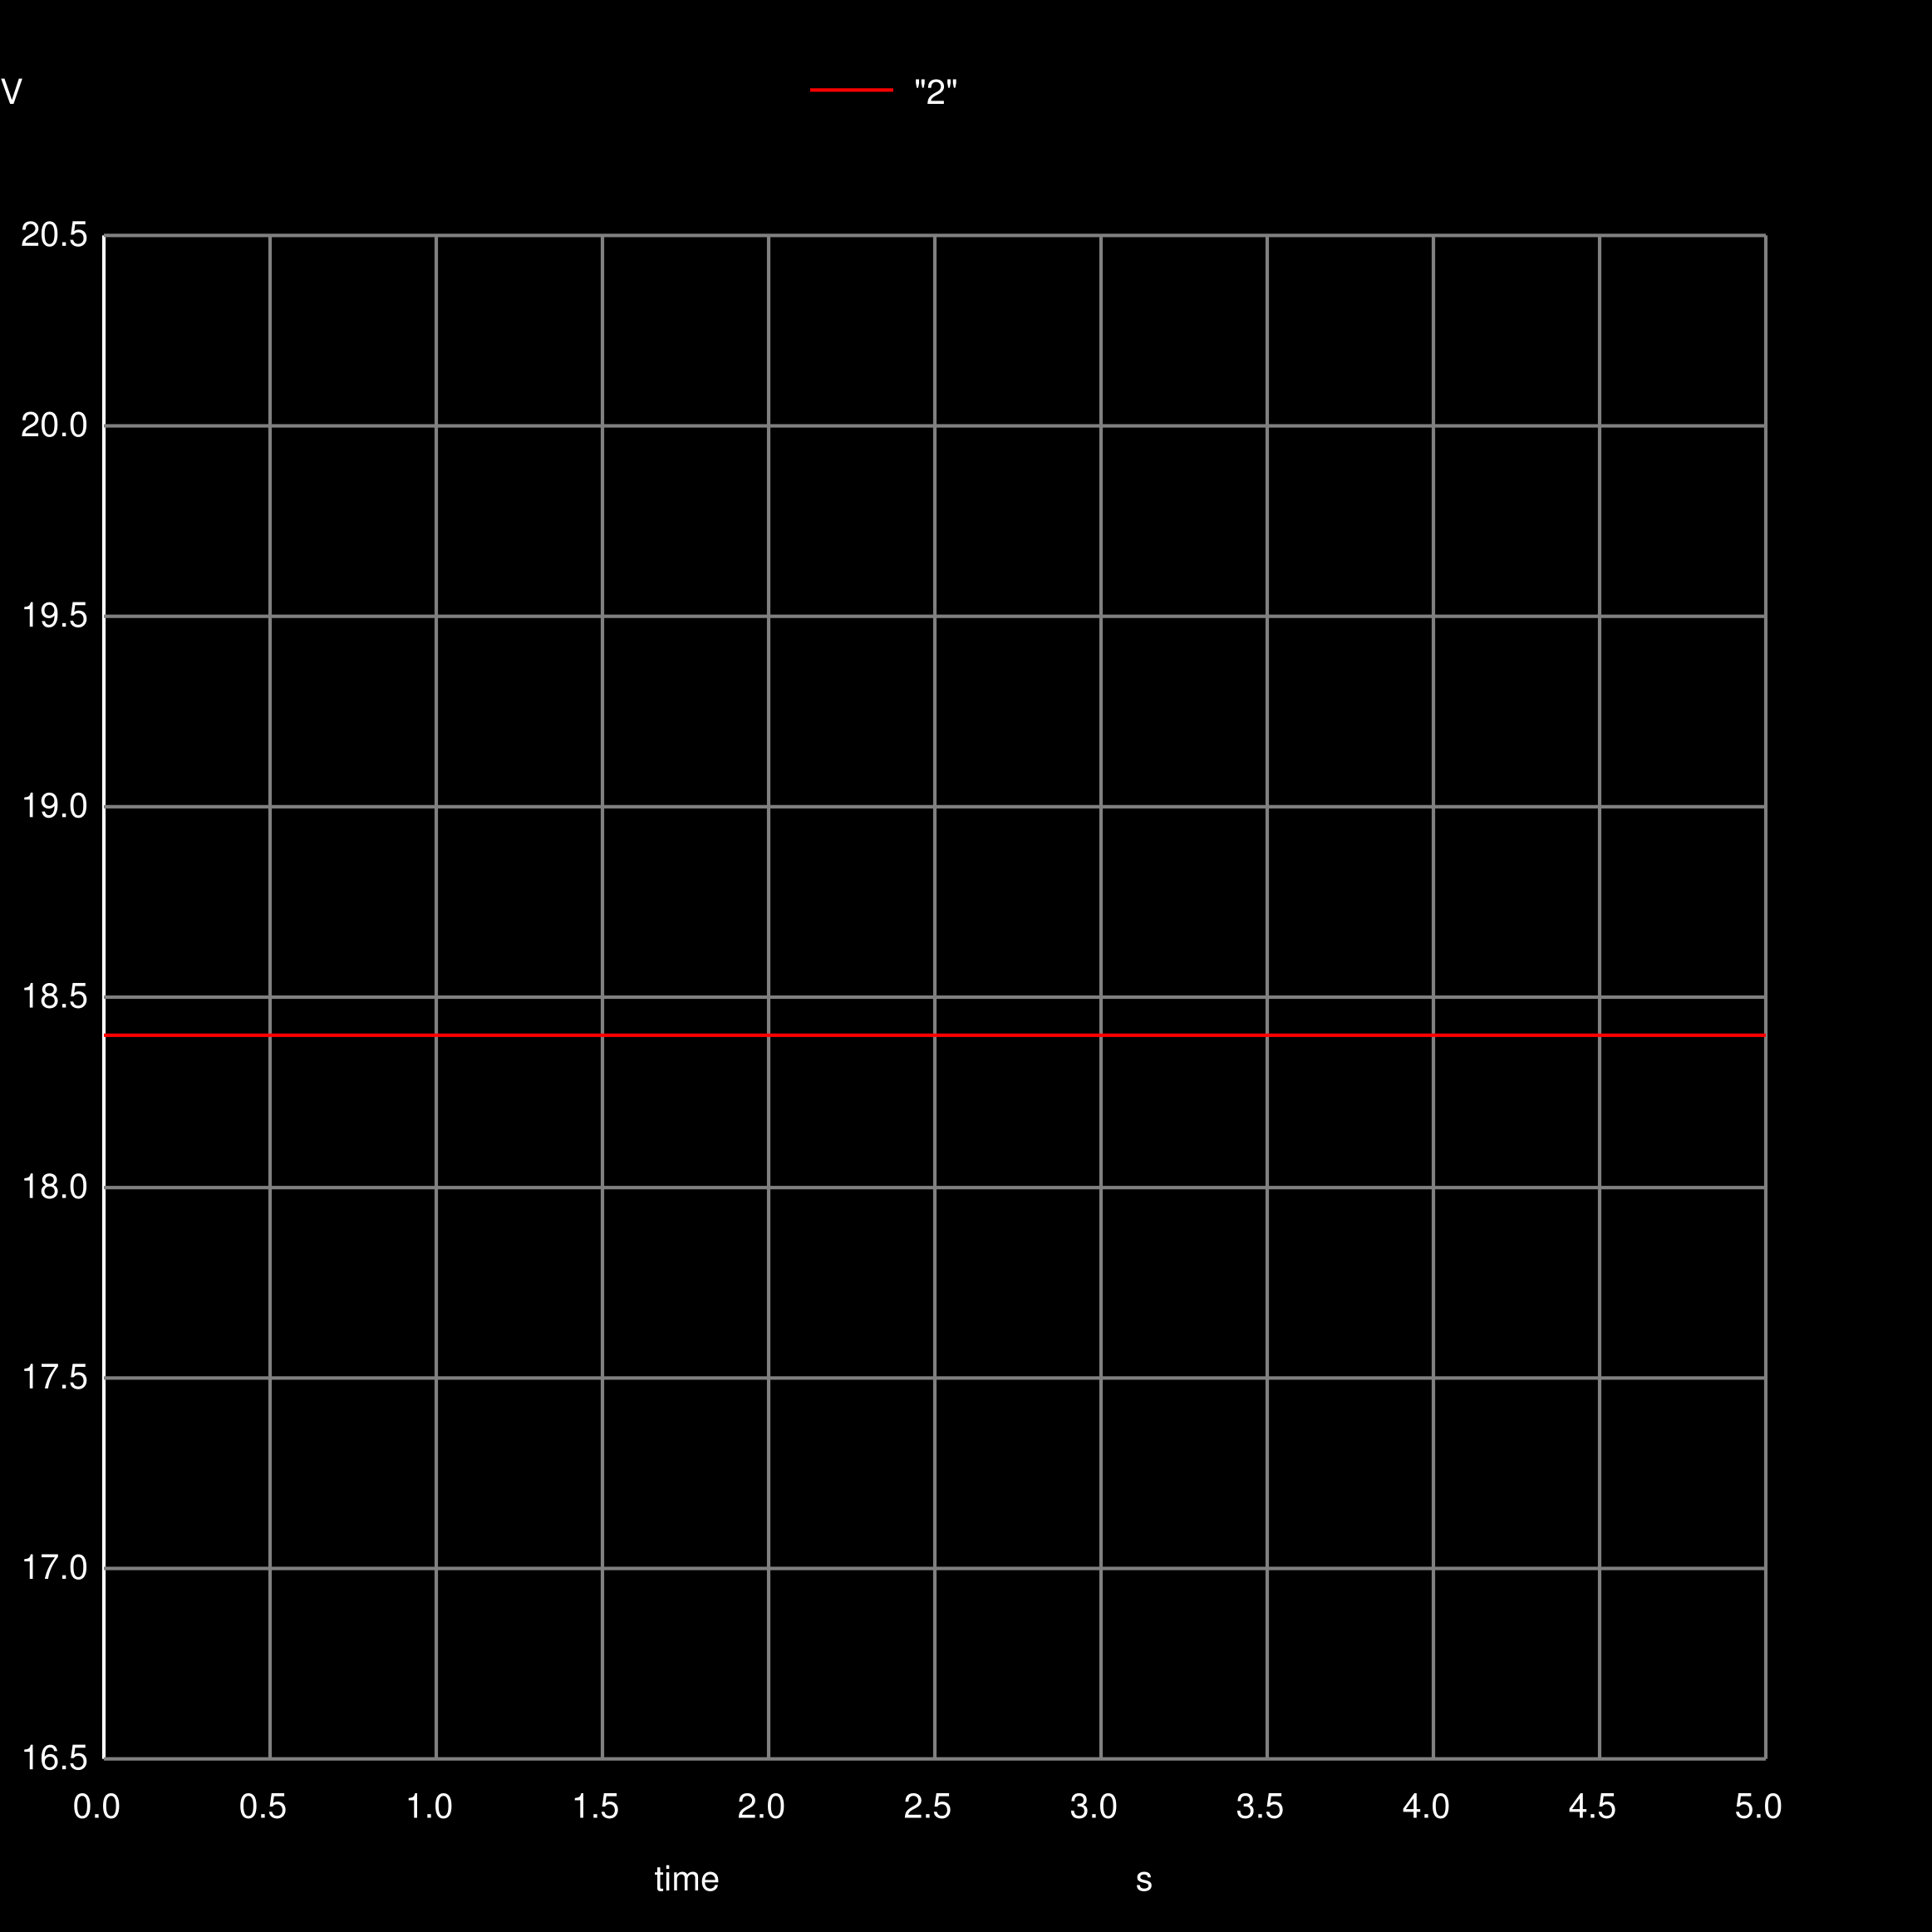
\includegraphics[width=\textwidth,height=\textheight,keepaspectratio]{IMAGES/012.png}
\caption{Grafiks no ngspice (2)}
\label{ngspice grafiks 2}
\end{figure}
\section{Darbs are QUCS programmām}
\subsection{Principāla shēma}
\begin{figure}[!tb]
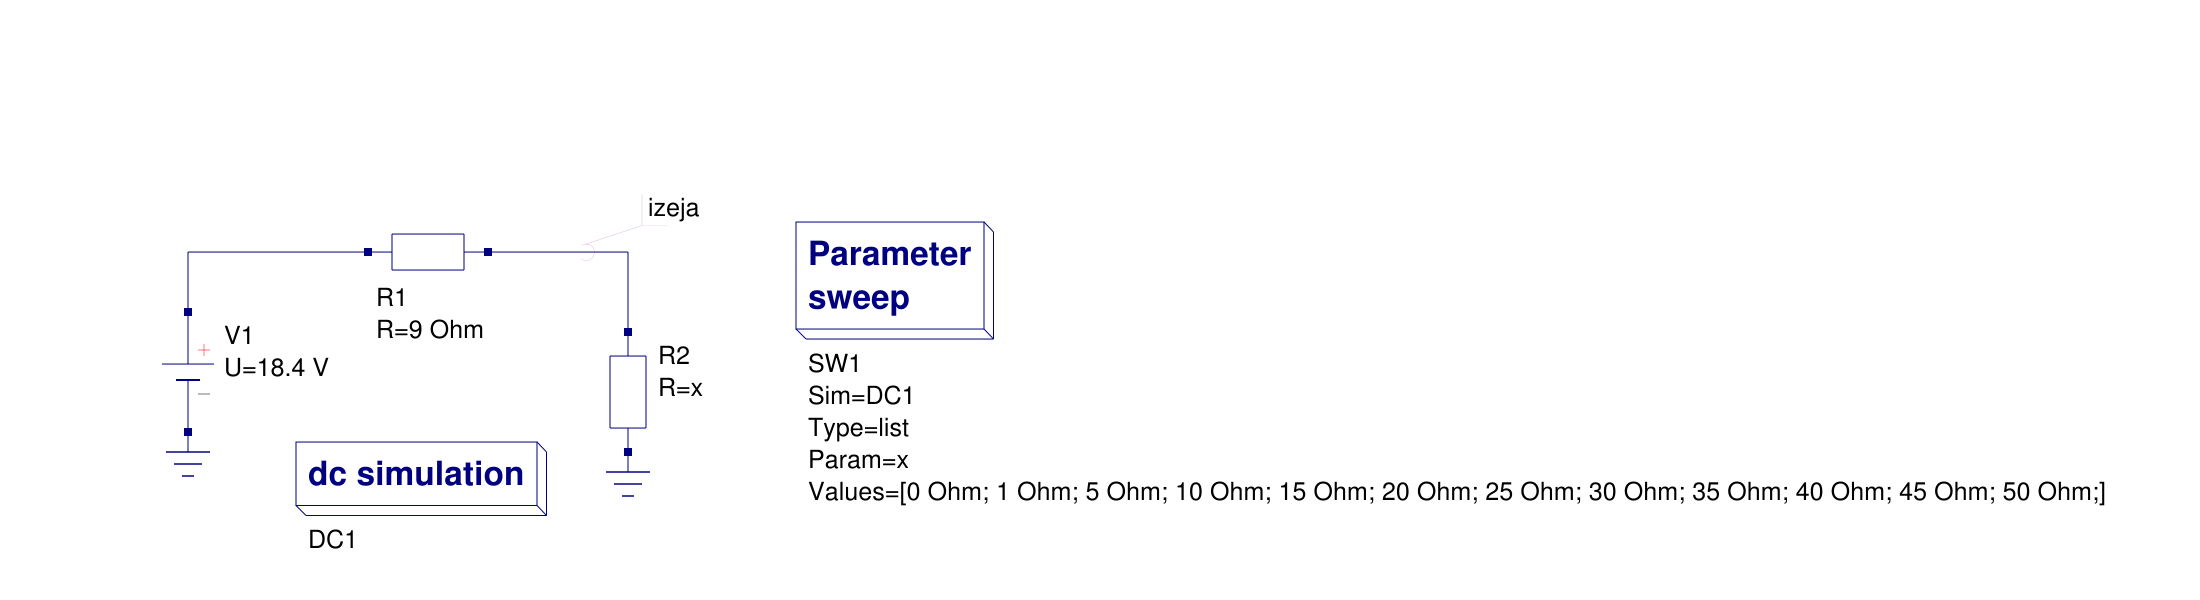
\includegraphics[width=\textwidth,height=\textheight,keepaspectratio]{IMAGES/02.png}
\caption{Principāla shēma}
\label{Principala shema}
\end{figure}
Shēma ar visiem elementiem, R2 ir aizvietots ar x lai to izmantot kā argumentu Parameter Sweep analīzē. (Att. \ref{Principala shema})
\subsection{Tabula un grafiks}
\begin{figure}[!tb]
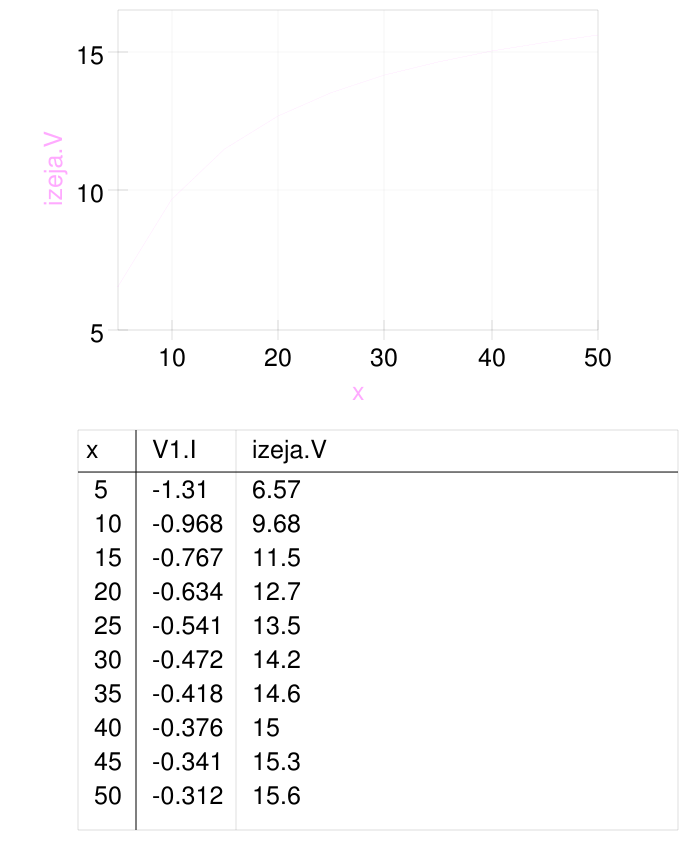
\includegraphics[width=\textwidth,height=\textheight,keepaspectratio]{IMAGES/02graphic.png}
\caption{Tabula un grafiks}
\label{Tabula un grafiks}
\end{figure}
no grafika spriegums uz R2 mainās proporcionāli R2 pretestības izmaiņai pret kopējo pretestību. (Att. \ref{Tabula un grafiks})
\begin{thebibliography}{9}
\bibitem{gramata1}
Andrejs Strauts. Elektrotehnikas teorētiskie pamati, lekciju konspekts. –Rīga,
RTU, 2008, -197 lpp.
\bibitem{gramata2}
Kārlis Brīvkalns. Ķēžu teorija. Vadonis Ķēžu teorijas studijām: praktiskās
nodarbības, laboratorijas darbi, MatLab programmas,PSpice pielietojums. –Rīga,
RTU, 2008, - 93 lpp.
\end{thebibliography}
\end{document}




